% Using 10pt, for IEEE journal form
% Final work
\documentclass[10pt, journal, final]{IEEEtran}

\usepackage[T1]{fontenc} 
\usepackage{amsmath}
\usepackage[cmintegrals]{newtxmath}
\usepackage{bm}
\usepackage{graphicx}
% Using mcode for input code of MATLAB
\usepackage{listings}
\usepackage[framed,numbered,autolinebreaks,useliterate]{mcode}

\markboth{IEEE TRANSACTIONS ON EDUCATION,~Vol.~X, No.~X, NOVEMBER~2020}%
{Qin \MakeLowercase{\textit{et al.}}: }

\begin{document}
\title{Engineering Electromagnetics - Experiment 2\\ Electric Field of Line Charge}
\author{\IEEEauthorblockN{Qingfu~Qin},
    \IEEEauthorblockA{Southern University of Science and Technology, ShengZhen, GuangDong}\\
    \IEEEauthorblockA{Email: 11910103@mail.sustech.edu.cn}
}

\maketitle

% abstract: electric field of line charge
% 1. Using MATLAB
% 2. Two methods: integration and infinitesimal
% 3. analyze difference
\begin{abstract}
    This article describes the electric field of the line charge which lenth is 2.
    By using MATLAB to simulate the electric field and draw the pictures;
    Using integration method to calculate the distribution of electric potential,
    the shape of electric field distribution is similar to the fin.
    Using infinitesimal method, divide line charge into 20, 50 and 100 segments,
    think of them as point charges, when increasing the degree of seperation, the
    electric field distribution is close to integration method.
    To analyze the difference between two methods, the difference caused by
    degree of seperation and the coordinate precision.
\end{abstract}

% Introduction part to describe the background of the experimnet
\section{
  Introduction
 }
\label{sec:Intro}

\IEEEPARstart{T}{his} experiment is to analyze the electric field of
the line charge in a free space. And the objectives of this experiment is:
\begin{itemize}
    \item Calculate the distribution of electric field
          built by continuous line charge
    \item Plot the relevant figures on MATLAB environment
    \item Study the difference betweenintegration and infinitesimal methodson
          on analyzing electric field.
\end{itemize}\par

By using the scientific analysis software MATLAB,
simulated the electric field distribution of
line charge in a 2-D rectangular coordinate can help us to
understand the electric field in a visualized way.\par

Suppose there is a uniformly distributed line charge
between point A(-1,0) and point B(1,0),
with line charge density of $\rho = 1 \times 10^{-9}$ C/m.
(The unit for the coordinate is m)\par

Using integration method in \ref{ method:integration }
to calculate the electric potential at each point of the coordinate,
we can get the real distribution in theory.
And using infinitesimal method in \ref{ method:infinitesimal }
to do a approximate simulation.\par

To describe the distribution, I use three graph included for each method.
They include:
\begin{itemize}
    \item i)   the distribution of electric field for each point;
    \item ii)  equipotential lines;
    \item iii) distribution of electric field lines(represented by continuous lines).
\end{itemize}\par
To analyze the difference, I calculate the difference of electric potential
between two ways at three different degree of seperation(20, 50 and 100).
Draw the graph of difference distribution.
And analyzed the difference at line: $y=0.5$,
using knowledge of calculus to describe the difference.

\section{
  Related Knowledge and Functions
 }
\label{sec:Related and Func}

In vaccuum, the electric field intensity ($\mathbf{E}$)
of a point charge can be expressed as:

\begin{equation}
    \mathbf{E} = k\frac{Q}{R^2}\mathbf{a}_R
\end{equation}

Where the coefficient $k = 9 \times 10^9$ F/m is the electrostatic constant.
$Q$ represent the total amount of charges. $R$ denotes the distance
between the point in the electric field and the source charge.\par

If we take reference point as the infinite distance, then the electric potential at
a point in the field is expressed as:
\begin{equation}
    V = k \frac{Q}{R}
\end{equation}

The electric field intensity can be expressed as the negative gradient of
the electric potential:
\begin{equation}
    \mathbf{E} = -\nabla V
\end{equation}

The electric field generated by N point charge in the vaccuum is expressed as:
\begin{equation}
    V = \sum_{i=1}^N k\frac{Q_i}{R_i}
\end{equation}

Similarly, the field magnitude generated by N point charges in the vaccuum can
be obtained through equation (3).\par

When the field source is continuous charge, e.g. line charge, we can readily resolve it
by using infinitesimal or integral method. the procedure of applying this method is
listed as follows:
\begin{itemize}
    \item 1) Divide the line charge into small segments of charges
          (usuallybeingdivided evenly).
    \item 2) Treat eachsmall segment of charges as a point charge and
          calculate the electric potential through equation (2).
    \item 3) Sum  up  all  the  electric  potential by using  equation  (4)
          to  obtain  the  electric potential.
    \item 4) Calculatethe electric field intensity generated by
          this line charge through equation (3).
\end{itemize}

\subsection{
    integration method
}\label{
    method:integration
}
Using integration method to calculate the distribution of electric potential
at each point of the coordinate, namely, the real distribution.
The procedure is given below:\\
Given a point $(X_0, Y_0)$:
\begin{equation}
    \begin{aligned}
        V= & \  k\int_{-1}^{1} \frac{\rho dx}{R}                                     \\
        =  & \ k\int_{-1}^{1} \frac{\rho dx}{\sqrt{(x-X_0)^2+Y_0^2}}                 \\
        =  & \ k \rho \ln{\left | (x-X_0)+\sqrt{(x-X_0)^2+Y_0^2} \right \|_{-1}^1  } \\
        =  & \  k \rho \ln{\left(
            \frac{1-X_0+\sqrt{(1-X_0)^2+Y_0^2}}{-1-X_0+\sqrt{(-1-X_0)^2+Y_0^2}}
            \right)}                                                                 \\
    \end{aligned}
\end{equation}

If we calculate each point of the coordinate.

\begin{equation}
    V(x,y)=k\rho\ln{\left(
        \frac{1-x+\sqrt{(1-x)^2+y^2}}{-1-x+\sqrt{(-1-x)^2+y^2}}
        \right)}
\end{equation}

Easy to prove, when calculated point is on the line charge, namely, $x\in[-1,1]$ and $y = 0$,
the electric potential is $\infty$.

\subsection{
    infinitesimal method
}\label{
    method:infinitesimal
}

Using infinitesimal method to calculate the distribution of electric potential
at each point of the coordinate, however, we cannot have infinitesimal in MATLAB,
so we use small segments as infinitesimal.\par
Set the approximative infinitesimal of distance is $\Delta x = \frac{l}{N}$.
Where l is the length of line charge $l = x_A - x_B = 2$, N is number of segments.
Using point charge to replace the segments,
so the x-coordinates are the midpoints of the segments.
Each x-coordinate is $x_i = i\frac{\Delta x}{2} + x_A = \frac{i}{N} - 1$
So, the approximate infinitesimal of charge is $\Delta Q = \rho \Delta x$.
According to equation (4), given a point $(X_0, Y_0)$:

\begin{equation}
    \begin{aligned}
        V = & \ \sum_{i=1}^N k\frac{\Delta Q}{R_i}                                             \\
        =   & \ k\rho \Delta x\sum_{i=1}^N \frac{1}{\sqrt{(x_i - X_0)^2+Y_0^2}}                \\
        =   & \ k\rho \frac{l}{N}\sum_{i=1}^N \frac{1}{\sqrt{(\frac{i}{N} - 1 - X_0)^2+Y_0^2}} \\
        =   & \ \frac{2k\rho}{N}
        \sum_{i=1}^N \frac{1}{\sqrt{(\frac{i}{N} - X_0 - 1)^2+Y_0^2}}                          \\
    \end{aligned}
\end{equation}

If we calculate each point of the coordinate.
\begin{equation}
    V(x,y) = \frac{2k\rho}{N}\sum_{i=1}^N \frac{1}{\sqrt{(\frac{i}{N} - x - 1)^2+y^2}} \\
\end{equation}

% MATLAB code 
\subsection{
    MATLAB Functions
}
\label{func}
Functions included:
\begin{itemize}
    \item 1) function: V\_con
    \item 2) function: V\_dis
\end{itemize}

% V_con for continuous calculate
\subsubsection*{
    V\_con
}
\label{V_con}
To calculate the electric field distribution
by using integration method, namely, it use equation (6) to calculate.
\lstinputlisting{../V_con.m}

% V_dis for descrete calculate
\subsubsection*{
    V\_dis
}
\label{V_dis}
To calculate the electric field distribution
by using infinitesimal method, namely, it use equation (8) to calculate.
\lstinputlisting{../V_dis.m}

% work 1
\section{
  Simulation of Integration Method
 }
 \label{sec:inte}
Using MATLAB to describe electric field and draw pictures
simulated by integration methods.\\
1. Initialization. Set the coordinates of 4m $\times$ 4m.
The number of coordinates is 60 $\times$ 60.
\lstinputlisting[lastline = 14]{../work1.m}
\label{work1.1}

2. Calculate the electric potential distributionby using \ref{func}: $V\_con$.
And draw picture of the distribution of electric field.
\lstinputlisting[firstline = 17, lastline =23]{../work1.m}
\label{work1.2}

\begin{figure}[htbp]
    \centering
    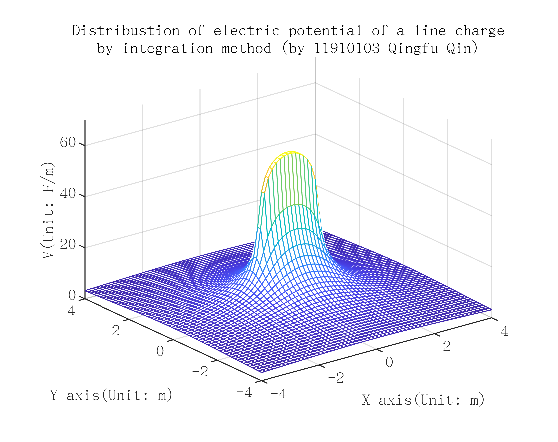
\includegraphics[width = 3.4in]{figures/fig1.1.eps}
    \caption{Distribution of electric potential simulated by integration method}
    \label{fig:1.1}
\end{figure}

As Figure~\ref{fig:1.1} shows that,
the distribution of electric potential is similar to shape of fins.
But for simulated by matlab,
the electric potential on the line charge is infinite in fact.\\
\\
\\
3. Draw picture of Isopotential lines.
Set range of potential is (0, 60) V.
\lstinputlisting[firstline = 26, lastline =36]{../work1.m}
\label{work1.3}
\begin{figure}[htbp]
    \centering
    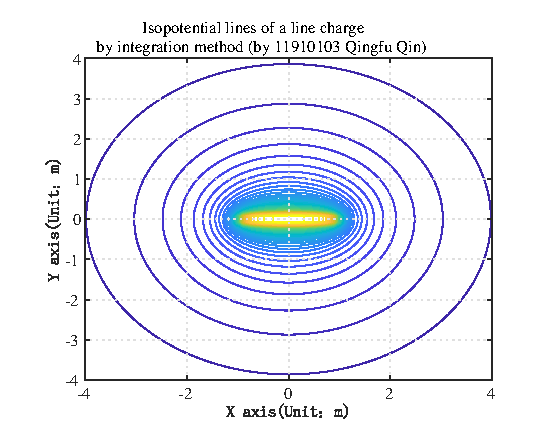
\includegraphics[width = 3.4in]{figures/fig1.2.eps}
    \caption{Isopotential lines simulated by integration method}
    \label{fig:1.2}
\end{figure}
As Figure~\ref{fig:1.2} shows that, the Isopotential lines are ellipse.
And when coordinate far from line charge, isopotential lines is being more round.
It is means that the potential distribution of a short line charge
is close to point charge in some ways.\\
\\
4. Draw picture of power lines.
\lstinputlisting[firstline = 39]{../work1.m}
\label{work1.4}
\begin{figure}[htbp]
    \centering
    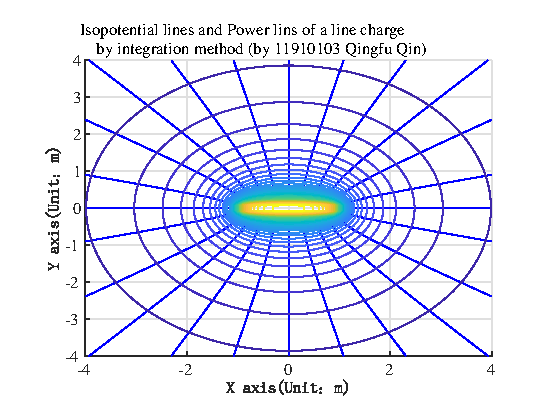
\includegraphics[width = 3.4in]{figures/fig1.3.eps}
    \caption{Isopotential lines simulated by integration method}
    \label{fig:1.3}
\end{figure}
As Figure~\ref{fig:1.3} shows that, power lines is flow outward from line charge.

% work 2
\section{
  Simulation of Infinitesimal Method
 }
 \label{sec:inf}
Using MATLAB to describe electric field and draw pictures
simulated by infinitesimal methods.\\
1. Initialization. Set the coordinates of 4m $\times$ 4m.
The number of coordinates is 60 $\times$ 60,
just similar to \ref{sec:inte}.
\lstinputlisting[lastline = 14]{../work1.m}
\label{work2.1}


\begin{lstlisting}
    for ni = n % darw 3 times picture for different n
        ...
        ...
        ...
    end
\end{lstlisting}

2. Calculate the electric potential distributionby using \ref{func}: $V\_con$.
And draw picture of the distribution of electric field.
\lstinputlisting[firstline = 17, lastline =23]{../work1.m}
\label{work1.3}

\begin{figure}[htbp]
    \centering
    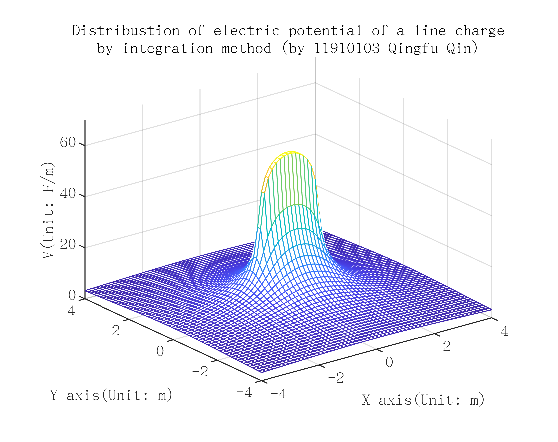
\includegraphics[width = 3.4in]{figures/fig1.1.eps}
    \caption{Distribution of electric potential simulated by integration method}
    \label{fig:1.1}
\end{figure}

As Figure~\ref{fig:1.1} shows that,
the distribution of electric potential is similar to shape of fins.
But for simulated by matlab,
the electric potential on the line charge is infinite in fact.\\
\\
\\
3. Draw picture of Isopotential lines.
Set range of potential is (0, 60) V.
\lstinputlisting[firstline = 26, lastline =36]{../work1.m}
\begin{figure}[htbp]
    \centering
    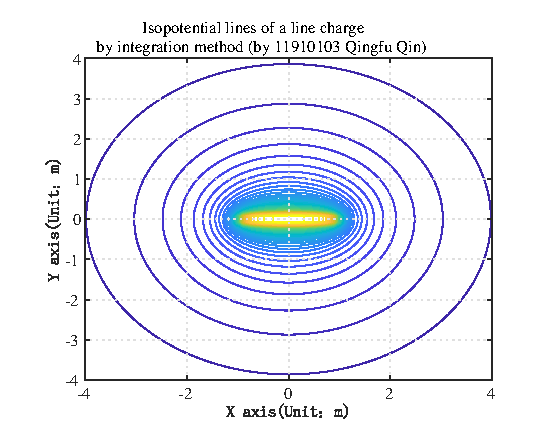
\includegraphics[width = 3.4in]{figures/fig1.2.eps}
    \caption{Isopotential lines simulated by integration method}
    \label{fig:1.2}
\end{figure}
As Figure~\ref{fig:1.2} shows that, the Isopotential lines are ellipse.
And when coordinate far from line charge, isopotential lines is being more round.
It is means that the potential distribution of a short line charge
is close to point charge in some ways.\\
\\
4. Draw picture of power lines.
\lstinputlisting[firstline = 39]{../work1.m}
\begin{figure}[htbp]
    \centering
    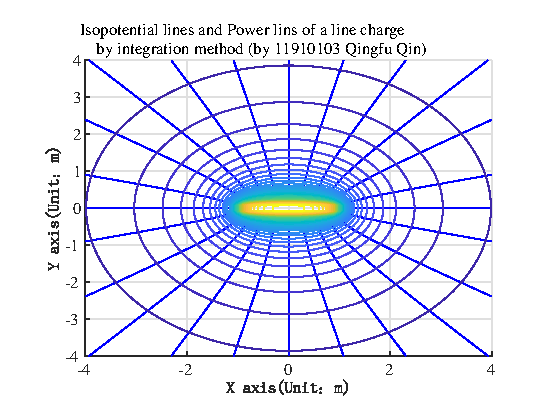
\includegraphics[width = 3.4in]{figures/fig1.3.eps}
    \caption{Isopotential lines simulated by integration method}
    \label{fig:1.3}
\end{figure}
As Figure~\ref{fig:1.3} shows that, power lines is flow outward from line charge.

\section*{Acknowledgment}
\thanks{
    Thanks to Youwei Jia, the teacher who teach me the knowledge about Electromagnetics
    and the using methods of MATLAB. He gives amounts of help to me to finish this article.
}


\end{document}